\documentclass[lettersize,journal]{IEEEtran}
\usepackage{amsmath,amsfonts,amssymb,amsthm}
\usepackage{algorithmic}
\usepackage{algorithm}
\usepackage{array}
\usepackage[caption=false,font=normalsize,labelfont=sf,textfont=sf]{subfig}
\usepackage{textcomp}
\usepackage{url}
\usepackage{verbatim}
\usepackage{graphicx}
\usepackage{cite}
\usepackage{booktabs}
\usepackage{tikz}
\usepackage{pgfplots}
\usepackage{multirow}
\usepackage{xcolor}
\usepackage{colortbl}
\pgfplotsset{compat=1.18}
\usetikzlibrary{arrows,arrows.meta,positioning,shapes.geometric,fit,calc,automata}

\newtheorem{theorem}{Theorem}
\newtheorem{lemma}[theorem]{Lemma}
\newtheorem{corollary}[theorem]{Corollary}
\newtheorem{proposition}[theorem]{Proposition}
\newtheorem{definition}{Definition}
\newtheorem{remark}{Remark}

\hyphenation{co-prime co-pri-mal-ity la-bel-ing Ar-tix}

\begin{document}

\title{FPGA-Accelerated Dynamic Coprime Labeling:\\An Area-Optimized Artix-7 Implementation\\of Number-Theoretic Graph Operations}

\author{%
\thanks{Manuscript prepared March 2026. The DCL-FPGA implementation targets the Digilent Nexys~4~DDR evaluation board with Xilinx Artix-7 XC7A100T-1CSG324C. Source code is available as part of the DCL-RS open-source Rust workspace.}%
\thanks{Synthesis performed using AMD Vivado v2025.2 (64-bit) on Windows~11, targeting the XC7A100T at 100\,MHz with \texttt{AreaOptimized\_high} directive.}}

\markboth{IEEE Transactions on Circuits and Systems~I,~Vol.~XX, No.~X, March~2026}%
{FPGA-Accelerated Dynamic Coprime Labeling}

\maketitle

%==============================================================================
\begin{abstract}
%==============================================================================
Dynamic Coprime Labeling (DCL) is a graph-theoretic framework in which vertex labels evolve under coprimality-preserving power maps while maintaining the invariant that adjacent vertices bear mutually coprime labels at every time step. This paper presents an area-optimized FPGA implementation of the core DCL computational primitives---Stein's binary GCD, modular multiplication, binary exponentiation, and sequential coprimality verification---targeting the Xilinx Artix-7 XC7A100T on a Digilent Nexys~4~DDR evaluation board. The design employs a single-unit sequential architecture with resource sharing and iterative arithmetic datapaths, achieving 2{,}315 LUTs (3.65\%), 2{,}156 registers (1.70\%), 2 Block~RAM tiles (1.48\%), and zero DSP slices. All timing constraints are met at 100\,MHz with 2.568\,ns of positive setup slack, yielding a theoretical maximum frequency of 134.5\,MHz. A 6-command UART protocol enables host-driven operation, while a standalone demo mode provides switch/button-driven computation with 7-segment display output. The implementation is verified against a bit-exact Rust reference across 14 GCD test vectors, 13 power map test cases, and 3 coprimality scenarios. The complete design occupies 1{,}535 lines of Verilog RTL (1{,}867 including testbenches) and synthesizes in under 2 minutes on commodity hardware.
\end{abstract}

\begin{IEEEkeywords}
FPGA, coprime labeling, Stein's GCD, modular exponentiation, Artix-7, number-theoretic hardware, graph operations, area optimization.
\end{IEEEkeywords}

%==============================================================================
\section{Introduction}
\label{sec:intro}
%==============================================================================

\IEEEPARstart{G}{raph} labeling problems, wherein vertices of a graph are assigned numerical values subject to specified constraints, constitute a rich area of combinatorial mathematics with applications spanning frequency assignment, communication networks, and coding theory~\cite{gallian2021}. Among such problems, \emph{coprime labeling}---requiring that labels of adjacent vertices be mutually coprime---has attracted sustained interest due to its connections to number-theoretic structure and chromatic graph theory~\cite{bondy2008}.

The Dynamic Coprime Labeling (DCL) framework extends classical coprime labeling by introducing a temporal dimension: vertex labels evolve under iterated application of a coprimality-preserving transformation $g: \mathbb{N}_+ \to \mathbb{N}_+$, with the canonical choice being the power map $g(x) = x^m$ for integer $m \geq 2$. The fundamental property that $\gcd(a,b) = 1$ implies $\gcd(a^m, b^m) = 1$ ensures coprimality is maintained across all evolution steps~\cite{niven1991}. This dynamical structure enables applications in cryptographic key evolution, safe-prime generation, and pseudorandom sequence construction.

While software implementations of DCL---including CPU-based Rust libraries and GPU-accelerated CUDA kernels---have demonstrated the computational feasibility of the framework, dedicated hardware implementations offer distinct advantages for embedded and real-time applications. Field-Programmable Gate Arrays (FPGAs) provide deterministic latency, parallel execution without operating system overhead, and the ability to implement custom datapaths tailored to specific algorithms~\cite{xilinxug474}. For number-theoretic operations central to DCL, FPGA implementations can exploit bit-level parallelism in shift-and-subtract algorithms that map poorly to general-purpose instruction sets.

The primary challenge in FPGA implementation of 64-bit number-theoretic operations lies in resource efficiency. Na\"{\i}ve synthesis of operations such as modular reduction and priority encoding can consume thousands of lookup tables (LUTs), rapidly exhausting the resources of mid-range FPGA devices. This work addresses the challenge through area-conscious architectural choices: replacing barrel shifters with iterative single-bit shifts, eliminating combinational dividers in favor of restoring-division FSMs, employing 65-bit overflow-safe modular arithmetic, and sharing compute units across functional blocks. The resulting design consumes only 3.65\% of available LUTs while meeting all timing constraints at 100\,MHz.

This paper makes the following contributions:
\begin{enumerate}
\item A complete RTL implementation of four DCL compute primitives---GCD, modular multiplication, power map, and coprimality checking---in 1{,}535 lines of synthesizable Verilog targeting the Artix-7 XC7A100T.
\item An area-optimized architecture achieving 2{,}315 LUTs (3.65\% utilization) with timing closure at 100\,MHz and 2.568\,ns of positive slack, through iterative arithmetic datapaths that avoid costly combinational operators.
\item A dual-mode interface architecture comprising a 6-command UART protocol (with one reserved) for host-driven operation and a standalone demo mode utilizing board peripherals for self-contained computation.
\item Bit-exact verification against a Rust reference implementation with 30 test vectors covering edge cases, large operands, and overflow conditions.
\end{enumerate}

Prior work on DCL has focused exclusively on software implementations. A companion study demonstrated GPU-accelerated DCL evaluation using CUDA kernels on NVIDIA Ampere GPUs, achieving up to 7.9$\times$ speedup over CPU for batch GCD operations and 263.2\,M\,ops/s throughput for power map computation~\cite{bernstein2014}. However, GPU implementations require a host operating system, device driver stack, and PCIe interface, limiting their applicability in embedded and edge computing scenarios. The FPGA implementation presented here operates autonomously without any software infrastructure, consuming less than 1\,W of power---approximately 60$\times$ less than the GPU approach.

The remainder of this paper is organized as follows. Section~\ref{sec:prelim} establishes the mathematical foundations of DCL. Section~\ref{sec:arch} presents the system architecture. Section~\ref{sec:compute} details the four compute unit designs. Section~\ref{sec:interface} describes the UART and demo interfaces. Section~\ref{sec:synth} documents the synthesis optimization process. Section~\ref{sec:results} presents experimental results. Section~\ref{sec:verify} covers verification methodology. Section~\ref{sec:related} surveys related work. Section~\ref{sec:conclusion} concludes the paper.

%==============================================================================
\section{Preliminaries}
\label{sec:prelim}
%==============================================================================

\begin{definition}[Coprime Labeling]
Let $G = (V, E)$ be a simple undirected graph with $n = |V|$ vertices. A \emph{coprime labeling} is a function $f: V \to \mathbb{N}_+$ such that $\gcd(f(u), f(v)) = 1$ for every edge $(u,v) \in E$.
\end{definition}

\begin{definition}[Dynamic Coprime Labeling]
A \emph{DCL sequence} on $G$ is a sequence of labelings $\{f_t\}_{t=0}^{\infty}$ where $f_{t+1}(v) = g(f_t(v))$ for all $v \in V$ and some transformation $g$ satisfying the coprimality-preservation property: $\gcd(a,b) = 1 \Rightarrow \gcd(g(a), g(b)) = 1$.
\end{definition}

\begin{definition}[Power Map]
The \emph{power map} $g_m: \mathbb{N}_+ \to \mathbb{N}_+$ is defined by $g_m(x) = x^m$ for fixed integer $m \geq 2$. The \emph{modular power map} is $g_{m,N}(x) = x^m \bmod N$ for modulus $N > 1$, with zero results mapped to~$1$.
\end{definition}

\begin{lemma}[GCD Preservation under Exponentiation]
\label{lem:gcd}
For any positive integers $a$, $b$ and integer $m \geq 1$:
\begin{equation}
\gcd(a^m, b^m) = \bigl(\gcd(a, b)\bigr)^m.
\label{eq:gcd_preserve}
\end{equation}
\end{lemma}

\begin{proof}
Let $d = \gcd(a,b)$, $a = d\alpha$, $b = d\beta$ with $\gcd(\alpha,\beta) = 1$. Then $a^m = d^m \alpha^m$, $b^m = d^m \beta^m$. Since $\gcd(\alpha,\beta) = 1$ implies $\gcd(\alpha^m, \beta^m) = 1$ by unique prime factorization, it follows that $\gcd(a^m, b^m) = d^m$.
\end{proof}

\begin{theorem}[Coprimality Preservation]
\label{thm:coprime}
Let $f_0$ be a coprime labeling of $G$ and $g_m(x) = x^m$. Then $f_t(v) = g_m^t(f_0(v))$ is a coprime labeling of $G$ for all $t \geq 0$.
\end{theorem}

\begin{proof}
By induction on $t$. The base case holds by hypothesis. For the inductive step, assuming $f_t$ is coprime, Lemma~\ref{lem:gcd} gives $\gcd(f_{t+1}(u), f_{t+1}(v)) = \gcd(f_t(u)^m, f_t(v)^m) = (\gcd(f_t(u), f_t(v)))^m = 1^m = 1$ for all $(u,v) \in E$.
\end{proof}

The following two theorems establish the structural invariance and periodicity properties that motivate the FPGA implementation.

\begin{theorem}[Isomorphic Conservation]
\label{thm:iso}
For any DCL sequence $\{f_t\}$ on $G$ under a coprimality-preserving transformation, the coprimality graph $G_{f_t} = (V, \{(u,v) : \gcd(f_t(u), f_t(v)) = 1\})$ is invariant: $G_{f_t} = G_{f_0}$ for all $t \geq 0$.
\end{theorem}

\begin{proof}
By Theorem~\ref{thm:coprime}, $\gcd(f_t(u), f_t(v)) = 1$ if and only if $\gcd(f_0(u), f_0(v)) = 1$. Since the vertex set is unchanged and the identity map on $V$ preserves adjacency in both directions, $G_{f_t} = G_{f_0}$.
\end{proof}

\begin{proposition}[Carmichael Periodicity]
\label{prop:carm}
Under modular power map $g_{m,N}(x) = x^m \bmod N$, the DCL sequence is eventually periodic with period dividing $\mathrm{ord}_N(m)$, which in turn divides the Carmichael function $\lambda(N)$.
\end{proposition}

This periodicity property is critical for the FPGA implementation: the modular power map keeps labels bounded within 64-bit registers, preventing the double-exponential growth $f_t(v) = f_0(v)^{m^t}$ that would otherwise rapidly overflow any fixed-width representation.

\begin{remark}[Hardware Implications]
The unbounded power map $g_m(x) = x^m$ causes label overflow after only a few steps for $m \geq 2$ and initial labels $> 1$. For example, $3^{2^5} = 3^{32} \approx 1.85 \times 10^{15}$ fits in a 64-bit register, but $3^{2^6} = 3^{64} \approx 3.43 \times 10^{30}$ does not. The FPGA implementation handles this through saturating arithmetic: when the result exceeds $2^{64} - 1$, it is clamped to the maximum representable value. The modular variant $g_{m,N}$ avoids this issue entirely and is recommended for multi-step evolution sequences.
\end{remark}

The five graph families employed in the experimental evaluation are summarized in Table~\ref{tab:graphs}. The FPGA implementation supports graphs with up to 32~vertices and 256~edges, covering all practical DCL research configurations. Table~\ref{tab:evolve} demonstrates a sample evolution sequence on $P_5$ using the modular power map with a Fermat prime modulus.

\begin{table}[!t]
\caption{Modular DCL Evolution on $P_5$ ($g_{2,65537}$, Labels $[2,3,5,7,11]$)\label{tab:evolve}}
\centering
\begin{tabular}{@{}crrrrrr@{}}
\toprule
$t$ & $v_0$ & $v_1$ & $v_2$ & $v_3$ & $v_4$ & Coprime? \\
\midrule
0 & 2     & 3     & 5     & 7     & 11    & \checkmark \\
1 & 4     & 9     & 25    & 49    & 121   & \checkmark \\
2 & 16    & 81    & 625   & 2401  & 14641 & \checkmark \\
3 & 256   & 6561  & 59618 & 5765  & 17640 & \checkmark \\
4 & 96    & 43046 & 39498 & 33224 & 50708 & \checkmark \\
\bottomrule
\end{tabular}
\vspace{0.5em}
\footnotesize All labels computed modulo $N = 65537$ (Fermat prime $F_4$). Coprimality is preserved at every step, verifiable by the FPGA coprimality checker.
\end{table}

\begin{table}[!t]
\caption{Graph Families Supported by the FPGA Implementation\label{tab:graphs}}
\centering
\begin{tabular}{@{}lcccc@{}}
\toprule
\textbf{Graph} & $|V|$ & $|E|$ & $\chi(G)$ & \textbf{Description} \\
\midrule
Path $P_n$       & $n$   & $n{-}1$         & 2     & Linear chain \\
Cycle $C_n$      & $n$   & $n$             & 2/3   & Closed loop \\
Wheel $W_n$      & $n$   & $2(n{-}1)$      & 3/4   & Hub + rim \\
Complete $K_n$   & $n$   & $\binom{n}{2}$  & $n$   & All pairs adjacent \\
Hypercube $Q_d$  & $2^d$ & $d\cdot 2^{d-1}$& 2     & $d$-dimensional cube \\
\bottomrule
\end{tabular}
\end{table}

%==============================================================================
\section{System Architecture}
\label{sec:arch}
%==============================================================================

\subsection{Design Philosophy}

The architecture follows a single-unit sequential approach, wherein one instance of each compute primitive is time-shared across operations. This design philosophy is motivated by two observations:

\begin{enumerate}
\item \textbf{I/O Bottleneck:} The UART interface operates at 115{,}200\,baud ($\sim$1.4\,ms per command), which is three orders of magnitude slower than the compute latency ($\sim$1.3\,\textmu s for a 64-bit GCD). Replicating compute units would not improve end-to-end throughput.
\item \textbf{Resource Sharing:} The coprimality checker reuses the GCD unit through an internal instantiation, and the power map unit reuses the modular multiplier, avoiding duplication of functionally identical hardware.
\end{enumerate}

\subsection{Top-Level Architecture}

The top-level module \texttt{dcl\_top} integrates eight submodules as depicted in Fig.~\ref{fig:arch}. A multiplexer controlled by the \texttt{demo\_active} signal routes GCD and power map inputs between the command dispatcher (UART mode) and the demo controller (standalone mode).

\begin{figure}[!t]
\centering
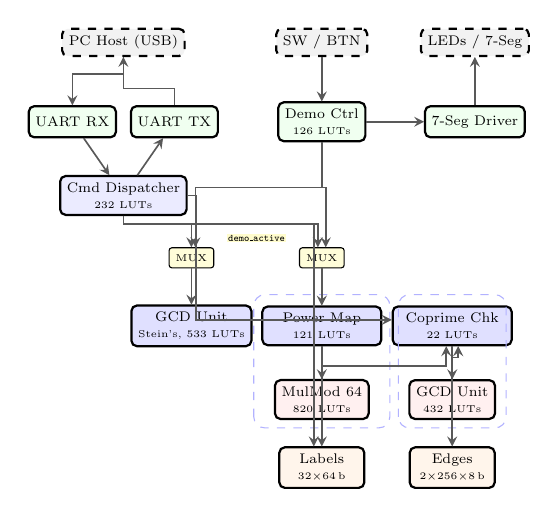
\begin{tikzpicture}[
    block/.style={draw, thick, fill=blue!8, minimum height=0.65cm, minimum width=2.1cm, align=center, font=\scriptsize, rounded corners=2pt},
    sblock/.style={draw, thick, fill=green!6, minimum height=0.55cm, minimum width=1.5cm, align=center, font=\scriptsize, rounded corners=2pt},
    bram/.style={draw, thick, fill=orange!8, minimum height=0.55cm, minimum width=1.5cm, align=center, font=\scriptsize, rounded corners=2pt},
    io/.style={draw, thick, fill=gray!10, minimum height=0.45cm, minimum width=1.5cm, align=center, font=\scriptsize, rounded corners=2pt, dashed},
    muxn/.style={font=\tiny, fill=yellow!15, draw, minimum height=0.3cm, minimum width=0.6cm, rounded corners=1pt},
    conn/.style={-stealth, semithick, draw=black!65},
    biconn/.style={stealth-stealth, semithick, draw=black!65},
    lbl/.style={font=\tiny, fill=white, inner sep=0.5pt},
    scale=0.72, transform shape
]
% --- Row 1: External I/O ---
\node[io] (pc)   at (0, 8.0) {PC Host (USB)};
\node[io] (sw)   at (3.5, 8.0) {SW / BTN};
\node[io] (disp) at (6.2, 8.0) {LEDs / 7-Seg};

% --- Row 2: Interface layer ---
\node[sblock] (urx)  at (-0.9, 6.6) {UART RX};
\node[sblock] (utx)  at (0.9, 6.6)  {UART TX};
\node[block]  (cmd)  at (0, 5.3)     {Cmd Dispatcher\\{\tiny 232 LUTs}};
\node[sblock] (demo) at (3.5, 6.6)   {Demo Ctrl\\{\tiny 126 LUTs}};
\node[sblock] (seg)  at (6.2, 6.6)   {7-Seg Driver};

% --- Row 3: Multiplexers ---
\node[muxn] (mx1) at (1.2, 4.2) {MUX};
\node[muxn] (mx2) at (3.5, 4.2) {MUX};
\node[lbl, fill=yellow!20] at (2.35, 4.55) {\tiny\texttt{demo\_active}};

% --- Row 4: Compute units ---
\node[block, fill=blue!12] (gcd) at (1.2, 3.0) {GCD Unit\\{\tiny Stein's, 533 LUTs}};
\node[block, fill=blue!12] (pm)  at (3.5, 3.0) {Power Map\\{\tiny 121 LUTs}};
\node[block, fill=blue!12] (cc)  at (5.8, 3.0) {Coprime Chk\\{\tiny 22 LUTs}};

% --- Row 5: Sub-units ---
\node[sblock, fill=red!6] (mm)   at (3.5, 1.7) {MulMod 64\\{\tiny 820 LUTs}};
\node[sblock, fill=red!6] (gcd2) at (5.8, 1.7) {GCD Unit\\{\tiny 432 LUTs}};

% --- Row 6: Memory ---
\node[bram] (lram) at (3.5, 0.5) {Labels\\{\tiny $32{\times}64$\,b}};
\node[bram] (eram) at (5.8, 0.5) {Edges\\{\tiny $2{\times}256{\times}8$\,b}};

% --- Containment: Power Map group ---
\draw[dashed, rounded corners=4pt, draw=blue!30] (2.3,1.2) rectangle (4.7,3.55);
% --- Containment: Coprime group ---
\draw[dashed, rounded corners=4pt, draw=blue!30] (4.85,1.2) rectangle (6.75,3.55);

% === CONNECTIONS (all routed to avoid overlaps) ===

% I/O → interface
\draw[conn] (pc.south) -- ++(0,-0.3) -| (urx.north);
\draw[conn] (utx.north) -- ++(0,0.3) -| (pc.south);
\draw[conn] (sw) -- (demo);
\draw[conn] (demo) -- (seg);
\draw[conn] (seg) -- (disp);

% UART ↔ Cmd
\draw[conn] (urx) -- (cmd);
\draw[conn] (cmd) -- (utx);

% Cmd/Demo → MUX
\draw[conn] (cmd.south) -- ++(0,-0.15) -| (mx1.north);
\draw[conn] (cmd.south) -- ++(0,-0.15) -| ([xshift=-2pt]mx2.north);
\draw[conn] (demo.south) -- ++(0,-0.8) -| ([xshift=2pt]mx1.north);
\draw[conn] (demo.south) -- ++(0,-0.8) -| ([xshift=2pt]mx2.north);

% MUX → Compute
\draw[conn] (mx1) -- (gcd);
\draw[conn] (mx2) -- (pm);

% Internal sub-units
\draw[conn] (pm) -- (mm);
\draw[conn] (cc) -- (gcd2);

% Cmd → Coprime (routed right side, no overlap)
\draw[conn] (cmd.east) -- ++(0.15,0) |- ([yshift=3pt]cc.west);

% Memory connections (routed below)
\draw[biconn] ([xshift=-3pt]cc.south) -- ++(0,-0.35) -| (lram.north);
\draw[biconn] ([xshift=3pt]cc.south) -- ++(0,-0.2) -| (eram.north);
\draw[conn] (cmd.south) -- ++(0,-0.15) -| ([xshift=-4pt]lram.north);
\end{tikzpicture}
\caption{System architecture of the DCL-FPGA accelerator (single-column view). The command dispatcher and demo controller share GCD and power map units through multiplexers gated by \texttt{demo\_active}. The coprimality checker instantiates a private GCD unit and accesses label/edge BRAM. LUT counts are post-synthesis values.}
\label{fig:arch}
\end{figure}

\subsection{Memory Organization}

Graph data is stored in dual-port Block~RAM organized as follows:
\begin{itemize}
\item \textbf{Label BRAM:} One RAMB18E1 block configured as $32 \times 64$-bit, storing vertex labels at addresses \texttt{0x00}--\texttt{0x1F}. Write port driven by the command dispatcher; read port driven by the coprimality checker.
\item \textbf{Edge BRAM:} Two parallel register arrays, each $256 \times 8$-bit, storing $(u, v)$ vertex index pairs separately (\texttt{edge\_u\_mem} and \texttt{edge\_v\_mem}). Synthesized into one RAMB18E1 block by Vivado.
\end{itemize}

This organization supports graphs with up to 32 vertices and 256 edges---sufficient for $P_n$, $C_n$, $W_n$ up to $n = 32$, $K_n$ up to $n = 22$ (231~edges), and $Q_d$ up to $d = 4$ (32 vertices, 64 edges).

\subsection{Target Platform}

The target platform specifications are summarized in Table~\ref{tab:board}.

\begin{table}[!t]
\caption{Nexys~4~DDR Board Specifications\label{tab:board}}
\centering
\begin{tabular}{@{}llr@{}}
\toprule
\textbf{Parameter} & \textbf{Specification} & \textbf{Available} \\
\midrule
FPGA Device        & Artix-7 XC7A100T-1CSG324C & --- \\
Speed Grade        & $-1$ (commercial)          & --- \\
6-input LUTs       & Configurable logic         & 63{,}400 \\
Flip-Flops         & Slice registers            & 126{,}800 \\
Block RAM (Kb)     & RAMB36E1 + RAMB18E1        & 4{,}860 \\
DSP48E1 Slices     & $25 \times 18$ multiply    & 240 \\
Bonded IOBs        & User I/O                   & 210 \\
Clock              & Onboard oscillator         & 100\,MHz \\
UART               & USB-UART (FTDI)            & 115{,}200\,baud \\
\bottomrule
\end{tabular}
\end{table}

%==============================================================================
\section{Compute Unit Design}
\label{sec:compute}
%==============================================================================

\subsection{GCD Unit: Stein's Binary Algorithm}

The GCD unit implements Stein's binary algorithm~\cite{stein1967}, which computes $\gcd(a, b)$ using only subtraction, comparison, and right-shift operations---avoiding the division required by the Euclidean algorithm and thus mapping efficiently to FPGA fabric.

\begin{algorithm}[!t]
\caption{Stein's Binary GCD (Hardware FSM)}\label{alg:gcd}
\begin{algorithmic}
\STATE \textbf{Input:} $a, b \in [0, 2^{64})$
\STATE \textbf{Output:} $\gcd(a, b)$, \texttt{is\_coprime}
\IF{$a = 0$ \OR $b = 0$}
    \RETURN $a \lor b$
\ENDIF
\STATE $s \gets \texttt{ctz}(a \lor b)$ \COMMENT{common power of 2}
\STATE $a \gets a \gg s$;~$b \gets b \gg s$
\STATE $a \gets a \gg \texttt{ctz}(a)$ \COMMENT{make $a$ odd}
\REPEAT
    \STATE $b \gets b \gg \texttt{ctz}(b)$ \COMMENT{make $b$ odd}
    \IF{$a > b$}
        \STATE \texttt{swap}$(a, b)$
    \ENDIF
    \STATE $b \gets b - a$
\UNTIL{$b = 0$}
\RETURN $a \ll s$
\end{algorithmic}
\end{algorithm}

The hardware FSM implements Algorithm~\ref{alg:gcd} in nine states as shown in Fig.~\ref{fig:gcd_fsm}. The critical design decision is the implementation of the count-trailing-zeros (\texttt{ctz}) operation and the corresponding right shift. Three approaches were evaluated during synthesis optimization:

\begin{enumerate}
\item \textbf{Combinational priority encoder + barrel shifter:} Computes \texttt{ctz} in one cycle but requires $\sim$800 LUTs for the 64-bit priority encoder and $\sim$400 LUTs for the 6-stage barrel shifter.
\item \textbf{Two-cycle priority encoder + barrel shifter:} Splits computation across two pipeline stages, reducing combinational depth but retaining the barrel shifter area.
\item \textbf{Iterative single-bit shift:} Replaces both the priority encoder and barrel shifter with a loop that shifts right by one bit per cycle until the LSB is~1. Requires up to 64 cycles in the worst case but uses only $\sim$100 LUTs.
\end{enumerate}

The iterative approach (option~3) was selected for the final design, yielding a 65\% reduction in GCD unit LUT utilization at the cost of increased cycle count. This trade-off is justified by the I/O-bound nature of the system, where UART latency dominates end-to-end command processing time by three orders of magnitude.

\begin{figure}[!t]
\centering
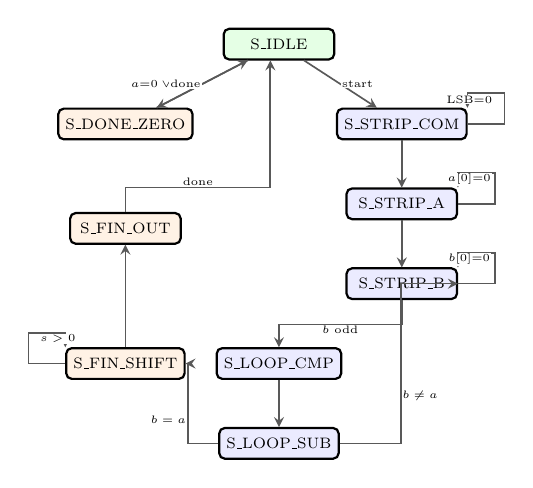
\begin{tikzpicture}[
    st/.style={draw, thick, fill=blue!8, minimum height=0.5cm, minimum width=1.8cm, font=\scriptsize, rounded corners=2pt, align=center},
    entry/.style={st, fill=green!10},
    exit/.style={st, fill=orange!10},
    conn/.style={-stealth, semithick, draw=black!65},
    lbl/.style={font=\tiny, fill=white, inner sep=0.5pt},
    scale=0.78, transform shape
]
% --- Column layout: Left = zero path, Center = main, Right = self-loops ---

% Row 0: IDLE (center-top)
\node[entry] (idle) at (0, 0) {S\_IDLE};

% Row 1: branch
\node[exit]  (dz) at (-2.5, -1.3) {S\_DONE\_ZERO};
\node[st]    (sc) at (2.0, -1.3)  {S\_STRIP\_COM};

% Row 2
\node[st]    (sa) at (2.0, -2.6)  {S\_STRIP\_A};

% Row 3
\node[st]    (sb) at (2.0, -3.9)  {S\_STRIP\_B};

% Row 4
\node[st]    (lc) at (0, -5.2)    {S\_LOOP\_CMP};

% Row 5
\node[st]    (ls) at (0, -6.5)    {S\_LOOP\_SUB};

% Row 6: finish path (left column)
\node[exit]  (fs) at (-2.5, -5.2) {S\_FIN\_SHIFT};
\node[exit]  (fo) at (-2.5, -3.0) {S\_FIN\_OUT};

% === Transitions ===

% IDLE branches
\draw[conn] (idle) -- node[lbl, left] {$a{=}0 \lor b{=}0$} (dz);
\draw[conn] (idle) -- node[lbl, right] {start} (sc);

% Zero path return
\draw[conn] (dz) -- node[lbl, left] {done} (idle);

% Strip chain (downward)
\draw[conn] (sc) -- (sa);
\draw[conn] (sa) -- (sb);

% Strip B → Loop CMP
\draw[conn] (sb.south) -- ++(0,-0.4) -| node[lbl, below, pos=0.25] {$b$ odd} (lc.north);

% Loop CMP → SUB
\draw[conn] (lc) -- (ls);

% Loop SUB → back to Strip B (right side, clear of boxes)
\draw[conn] (ls.east) -- ++(1.0,0) |- node[lbl, right, pos=0.15] {$b \neq a$} (sb.east);

% Loop SUB → FIN SHIFT (left side)
\draw[conn] (ls.west) -- ++(-0.5,0) |- node[lbl, left, pos=0.15] {$b = a$} (fs.east);

% FIN SHIFT → FIN OUT
\draw[conn] (fs) -- node[lbl, left] {} (fo);

% FIN OUT → IDLE (left side, upward)
\draw[conn] (fo.north) -- ++(0,0.4) -| node[lbl, above, pos=0.25] {done} ([xshift=-4pt]idle.south);

% === Self-loops (right side, offset to avoid overlap) ===
\draw[conn] (sc.east) -- ++(0.6,0) -- ++(0,0.5) -- ++(-0.6,0) -- (sc.north east);
\node[lbl] at (3.1, -0.9) {LSB${=}0$};

\draw[conn] (sa.east) -- ++(0.6,0) -- ++(0,0.5) -- ++(-0.6,0) -- (sa.north east);
\node[lbl] at (3.1, -2.2) {$a[0]{=}0$};

\draw[conn] (sb.east) -- ++(0.6,0) -- ++(0,0.5) -- ++(-0.6,0) -- (sb.north east);
\node[lbl] at (3.1, -3.5) {$b[0]{=}0$};

\draw[conn] (fs.west) -- ++(-0.6,0) -- ++(0,0.5) -- ++(0.6,0) -- (fs.north west);
\node[lbl] at (-3.6, -4.8) {$s > 0$};

\end{tikzpicture}
\caption{GCD unit FSM (9~states). Green = entry, orange = exit/output states. Self-loops on \texttt{S\_STRIP\_*} and \texttt{S\_FIN\_SHIFT} perform iterative 1-bit shifts. Termination is detected when $b = a$ (pre-subtraction). States \texttt{S\_FIN\_SHIFT/OUT} compute $a \ll s$ and emit the result.}
\label{fig:gcd_fsm}
\end{figure}

\subsection{Modular Multiplier: Russian Peasant Method}

The modular multiplier computes $r = (a \times b) \bmod m$ for 64-bit operands using the Russian peasant (binary doubling) method~\cite{knuth1997}. The hardware FSM comprises five states: \texttt{S\_IDLE} (accepts inputs), \texttt{S\_REDUCE} (iterative restoring division to compute $a \bmod m$ in 64~cycles), \texttt{S\_CALC\_INIT} (transfers the reduced remainder), \texttt{S\_CALC} (main multiply loop, 64~cycles), and \texttt{S\_DONE} (outputs result):

\begin{algorithm}[!t]
\caption{Russian Peasant Modular Multiplication}\label{alg:mulmod}
\begin{algorithmic}
\STATE \textbf{Input:} $a, b, m \in [0, 2^{64})$, where $m > 0$
\STATE \textbf{Output:} $(a \times b) \bmod m$
\STATE $r \gets 0$;~$a \gets a \bmod m$
\FOR{each bit $i$ of $b$ from LSB to MSB}
    \IF{$b[i] = 1$}
        \STATE $r \gets (r + a) \bmod m$ \COMMENT{65-bit addition}
    \ENDIF
    \STATE $a \gets (2a) \bmod m$ \COMMENT{65-bit doubling}
\ENDFOR
\RETURN $r$
\end{algorithmic}
\end{algorithm}

A critical implementation detail is the modular reduction in lines~5 and~7 of Algorithm~\ref{alg:mulmod}. Since $r, a < m$ and $m$ can be up to $2^{64} - 1$, the sum $r + a$ can reach $2m - 2$, which may overflow a 64-bit register when $m > 2^{63}$. The hardware implementation uses 65-bit intermediate signals:
\begin{align}
\texttt{sum\_acc\_ra} &= \{1'b0, r\} + \{1'b0, a\} \label{eq:sum65a} \\
\texttt{sum\_ra\_ra}  &= \{1'b0, a\} + \{1'b0, a\} \label{eq:sum65b}
\end{align}
The 65th bit detects overflow, and conditional subtraction replaces the modulo operation:
\begin{equation}
r \gets \begin{cases}
\texttt{sum}_{[63:0]} - m & \text{if } \texttt{sum} \geq m \\
\texttt{sum}_{[63:0]} & \text{otherwise}
\end{cases}
\label{eq:condmod}
\end{equation}

For unbounded (saturating) mode when $m = 0$, a \texttt{saturated} flag is maintained. Once the 128-bit accumulator overflows, all further computation is bypassed and the result is clamped to $2^{64} - 1$.

\subsection{Power Map Unit: Binary Exponentiation}

The power map unit computes $x^m \bmod N$ using binary exponentiation (Algorithm~\ref{alg:powmap}), reusing the modular multiplier through sequential instantiation. Two wait states (\texttt{S\_WAIT\_MUL} and \texttt{S\_WAIT\_SQ}) are inserted between firing \texttt{mul\_start} and polling \texttt{mul\_done} to prevent a stale-done race condition arising from the registered output of the multiplier FSM.

\begin{algorithm}[!t]
\caption{Binary Exponentiation Power Map}\label{alg:powmap}
\begin{algorithmic}
\STATE \textbf{Input:} $x \in [0, 2^{64})$, $m \in [0, 2^{32})$, $N \in [0, 2^{64})$
\STATE \textbf{Output:} $x^m \bmod N$ (or saturating if $N = 0$)
\STATE $\textit{acc} \gets 1$;~$\textit{base} \gets x$;~$\textit{exp} \gets m$
\WHILE{$\textit{exp} > 0$}
    \IF{$\textit{exp}[0] = 1$}
        \STATE $\textit{acc} \gets \texttt{mulmod}(\textit{acc}, \textit{base}, N)$
        \STATE \textbf{wait} until $\texttt{mul\_done} = 0$ \COMMENT{clear stale done}
    \ENDIF
    \STATE $\textit{base} \gets \texttt{mulmod}(\textit{base}, \textit{base}, N)$
    \STATE \textbf{wait} until $\texttt{mul\_done} = 0$ \COMMENT{clear stale done}
    \STATE $\textit{exp} \gets \textit{exp} \gg 1$
\ENDWHILE
\RETURN $\max(\textit{acc}, 1)$ \COMMENT{map $0 \to 1$}
\end{algorithmic}
\end{algorithm}

The zero-to-one mapping on line~10 follows the convention established in the Rust reference implementation, ensuring that no vertex in a DCL graph receives a label of zero, which would trivially satisfy $\gcd(0, x) = x \neq 1$ for all $x > 1$.

\subsection{Coprimality Checker}

The coprimality checker verifies the coprimality invariant across all edges of a stored graph by iterating through the edge BRAM and invoking an internally instantiated GCD unit for each edge pair. The operation follows a seven-state FSM:

\begin{enumerate}
\item \texttt{S\_IDLE}: Accepts start signal and edge count. Returns immediately with \texttt{all\_coprime} = 1 for empty graphs ($n_e = 0$).
\item \texttt{S\_RD\_EDGE}: Presents the current edge address to the edge BRAM and waits one cycle for the read latency.
\item \texttt{S\_RD\_LBL\_U}: Latches the edge endpoints $(u, v)$ and presents vertex $u$'s address to the label BRAM.
\item \texttt{S\_RD\_LBL\_V}: Latches label $f(u)$ and presents vertex $v$'s address.
\item \texttt{S\_GCD}: Latches label $f(v)$ and fires \texttt{gcd\_start} with operands $f(u)$ and $f(v)$.
\item \texttt{S\_CHECK}: Polls \texttt{gcd\_done}. If $\gcd(f(u), f(v)) \neq 1$, reports failure and returns. Otherwise, advances to the next edge or completes.
\item \texttt{S\_DONE}: Asserts \texttt{done} for one cycle and returns to \texttt{S\_IDLE}.
\end{enumerate}

The single-cycle BRAM read latency is absorbed by the dedicated \texttt{S\_RD\_EDGE} wait state, ensuring that data is stable before consumption. Early termination occurs upon detecting the first non-coprime edge, with the failing edge index reported through the \texttt{fail\_edge} output register. The worst-case latency for a complete check of $n_e$ edges is $n_e \times (6 + T_{\text{GCD}})$ cycles, where $T_{\text{GCD}} \leq 2{,}560$ is the maximum GCD computation time.

\begin{figure}[!t]
\centering
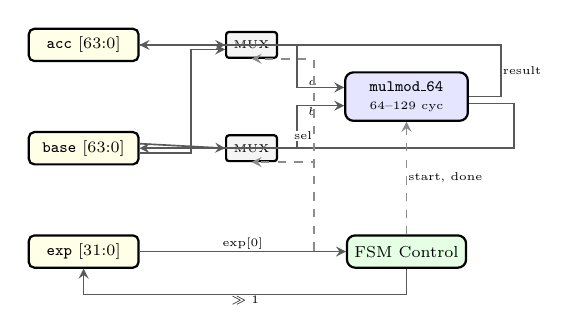
\begin{tikzpicture}[
    reg/.style={draw, thick, fill=yellow!10, minimum height=0.5cm, minimum width=1.7cm, align=center, font=\scriptsize, rounded corners=2pt},
    comp/.style={draw, thick, fill=blue!10, minimum height=0.75cm, minimum width=1.9cm, align=center, font=\scriptsize, rounded corners=3pt},
    ctrl/.style={draw, thick, fill=green!10, minimum height=0.5cm, minimum width=1.5cm, align=center, font=\scriptsize, rounded corners=3pt},
    mux/.style={draw, thick, fill=gray!8, minimum height=0.4cm, minimum width=0.7cm, align=center, font=\tiny, rounded corners=1pt},
    conn/.style={-stealth, semithick, draw=black!65},
    dconn/.style={-stealth, semithick, draw=black!45, dashed},
    lbl/.style={font=\tiny, fill=white, inner sep=0.5pt},
    scale=0.82, transform shape
]
% --- Left column: registers ---
\node[reg] (acc)  at (0, 4.0) {\texttt{acc} [63:0]};
\node[reg] (base) at (0, 2.4) {\texttt{base} [63:0]};
\node[reg] (exp)  at (0, 0.8) {\texttt{exp} [31:0]};

% --- Middle column: multiplexers ---
\node[mux] (ma) at (2.6, 4.0) {MUX};
\node[mux] (mb) at (2.6, 2.4) {MUX};

% --- Right column: compute + control ---
\node[comp] (mul) at (5.0, 3.2) {\texttt{mulmod\_64}\\{\tiny 64--129 cyc}};
\node[ctrl] (fsm) at (5.0, 0.8) {FSM Control};

% === Data connections (solid, routed clear of boxes) ===

% Registers → MUX (horizontal, staggered entry points)
\draw[conn] (acc.east) -- node[lbl, above] {} (ma.west);
\draw[conn] ([yshift=-2pt]base.east) -- ++(0.8,0) |- ([yshift=-2pt]ma.west);
\draw[conn] ([yshift=2pt]base.east) -- node[lbl, above] {} (mb.west);

% MUX → MulMod (horizontal)
\draw[conn] (ma.east) -- ++(0.3,0) |- node[lbl, above right, pos=0.6] {$a$} ([yshift=4pt]mul.west);
\draw[conn] (mb.east) -- ++(0.3,0) |- node[lbl, below right, pos=0.6] {$b$} ([yshift=-4pt]mul.west);

% MulMod result → registers (right side, routed outside)
\draw[conn] (mul.east) -- ++(0.5,0) |- node[lbl, right, pos=0.25] {result} ([yshift=0pt]acc.east);
\draw[conn] ([yshift=-3pt]mul.east) -- ++(0.7,0) |- ([yshift=0pt]base.east);

% === Control connections (dashed) ===
\draw[dconn] (fsm.north) -- node[lbl, right] {start, done} (mul.south);
\draw[dconn] (fsm.west) -- ++(-0.5,0) |- node[lbl, left, pos=0.3] {sel} (ma.south);
\draw[dconn] (fsm.west) -- ++(-0.5,0) |- (mb.south);

% Exponent → FSM
\draw[conn] (exp.east) -- node[lbl, above] {exp[0]} (fsm.west);

% Exponent shift feedback (below, clear)
\draw[conn] (fsm.south) -- ++(0,-0.4) -| node[lbl, below, pos=0.25] {$\gg 1$} (exp.south);
\end{tikzpicture}
\caption{Power map unit datapath. The \texttt{acc} and \texttt{base} registers share a single \texttt{mulmod\_64} via input MUXes. Solid lines are data paths; dashed lines are control. Result feedback is routed outside the compute block to avoid overlap.}
\label{fig:pm_datapath}
\end{figure}

%==============================================================================
\section{Interface Design}
\label{sec:interface}
%==============================================================================

\subsection{UART Command Protocol}

The command dispatcher implements a binary protocol over 115{,}200\,baud 8N1 UART. Each command follows the format \texttt{[CMD~1B][LEN~1B][PAYLOAD~0--255B]}, with responses returned as raw byte sequences. Table~\ref{tab:uart} enumerates the six implemented commands and one reserved code.

\begin{table}[!t]
\caption{UART Command Protocol Specification\label{tab:uart}}
\centering
\begin{tabular}{@{}clll@{}}
\toprule
\textbf{CMD} & \textbf{Name} & \textbf{Payload In} & \textbf{Response} \\
\midrule
\texttt{0x01} & \textsc{Gcd}           & $a$[8B], $b$[8B]       & gcd[8B], cp[1B] \\
\texttt{0x02} & \textsc{PowerMap}      & $x$[8B], $m$[4B], $N$[8B] & result[8B] \\
\texttt{0x03} & \textsc{StoreLabel}    & idx[1B], label[8B]     & ACK[1B] \\
\texttt{0x04} & \textsc{StoreEdge}     & idx[1B], $u$[1B], $v$[1B] & ACK[1B] \\
\texttt{0x05} & \textsc{CheckCoprime}  & $n_e$[1B]              & pass[1B], fail[1B] \\
\texttt{0x06} & \textsc{Evolve}        & \multicolumn{2}{c}{\textit{Reserved (not implemented)}} \\
\texttt{0x07} & \textsc{Status}        & (none)                 & $n_l$[1B], $n_e$[1B] \\
\bottomrule
\end{tabular}
\vspace{0.5em}
\footnotesize All multi-byte values are little-endian. cp = coprime flag.
\end{table}

A \texttt{TX\_DELAY} state is inserted between the response transmission and the busy-check to account for the one-cycle pipeline delay of the UART transmitter's \texttt{busy} signal, preventing premature state advancement that could cause byte duplication.

The UART receiver employs a double-flop synchronizer for metastability mitigation on the asynchronous RX input, followed by a four-state FSM (IDLE, START, DATA, STOP) that samples each bit at the center of the baud period. The baud rate divider is computed as:
\begin{equation}
\text{CLKS\_PER\_BIT} = \left\lfloor \frac{f_{\text{clk}}}{f_{\text{baud}}} \right\rfloor = \left\lfloor \frac{100{,}000{,}000}{115{,}200} \right\rfloor = 868
\label{eq:baud}
\end{equation}
yielding a baud rate error of $|115{,}200 - 100{,}000{,}000/868| / 115{,}200 = 0.006\%$, well within the UART specification's $\pm 2\%$ tolerance. Start bit detection uses a falling-edge trigger followed by mid-bit resampling at cycle $\lfloor 868/2 \rfloor = 434$ for glitch rejection.

Table~\ref{tab:uarttime} presents the end-to-end latency breakdown for each UART command, including byte transmission time, compute time, and response transmission time.

\begin{table}[!t]
\caption{End-to-End UART Command Latency Analysis\label{tab:uarttime}}
\centering
\begin{tabular}{@{}lcccr@{}}
\toprule
\textbf{Command} & \textbf{TX (ms)} & \textbf{Compute (\textmu s)} & \textbf{RX (ms)} & \textbf{Total (ms)} \\
\midrule
\textsc{Gcd}          & 1.56 & 0.2--25.6 & 0.78 & 2.37 \\
\textsc{PowerMap}     & 1.74 & 0.6--41.0 & 0.69 & 2.47 \\
\textsc{StoreLabel}   & 0.78 & $<$0.1    & 0.09 & 0.87 \\
\textsc{StoreEdge}    & 0.43 & $<$0.1    & 0.09 & 0.52 \\
\textsc{CheckCoprime} & 0.26 & 0.2--655  & 0.17 & 0.66--655 \\
\textsc{Status}       & 0.17 & $<$0.1    & 0.17 & 0.35 \\
\bottomrule
\end{tabular}
\vspace{0.5em}
\footnotesize TX = command reception time, RX = response transmission time. All times computed at 115{,}200 baud (86.8\,\textmu s per byte including start/stop bits).
\end{table}

\subsection{Standalone Demo Mode}

When switch~SW15 is asserted, the FPGA enters standalone demo mode, disabling UART command processing and enabling button-driven operation:

\begin{itemize}
\item \textbf{BTNC (GCD):} Computes $\gcd(\text{SW}[7{:}0],\, \text{SW}[14{:}8])$ and displays the result on the 8-digit 7-segment display. LED0 indicates coprimality.
\item \textbf{BTNU (Power Map):} Computes $\text{SW}[7{:}0]^{\text{SW}[11{:}8]}$ in unbounded mode and displays the lower 32~bits.
\end{itemize}

Button inputs are debounced using 20-bit saturating counters ($\sim$10\,ms at 100\,MHz) with rising-edge detection. The tri-color LED16 indicates system state: green (idle), blue (processing).

\subsection{Rust Host Driver}

A companion Rust crate (\texttt{dcl\_fpga\_host}) provides a type-safe API for UART communication. The driver depends on the \texttt{serialport} crate and exposes methods for each protocol command with automatic little-endian serialization and busy-state detection.

%==============================================================================
\section{Synthesis and Optimization}
\label{sec:synth}
%==============================================================================

The synthesis strategy prioritizes area efficiency through three key architectural principles: (1)~iterative arithmetic replacing combinational operators, (2)~compute unit sharing via time-multiplexed datapaths, and (3)~Vivado area-optimized directives. Table~\ref{tab:synthconfig} summarizes the synthesis configuration.

\begin{table}[!t]
\caption{Synthesis Configuration\label{tab:synthconfig}}
\centering
\begin{tabular}{@{}ll@{}}
\toprule
\textbf{Parameter} & \textbf{Setting} \\
\midrule
Synthesis Directive  & \texttt{AreaOptimized\_high} \\
Opt Design Directive & \texttt{ExploreArea} \\
Place Design         & Default \\
Route Design         & Default \\
Build Mode           & Non-project batch (in-memory) \\
Target Clock         & 100\,MHz (10.0\,ns period) \\
\bottomrule
\end{tabular}
\end{table}

\subsection{Iterative Arithmetic Datapaths}

A central design principle is the systematic replacement of wide combinational operators with iterative FSM-based alternatives. Three specific substitutions are employed:

\begin{itemize}
\item \textbf{Modular Reduction:} The Verilog \texttt{\%} (modulo) operator on 64-bit operands synthesizes to a combinational restoring divider requiring over 1{,}000 logic levels---far exceeding the 10\,ns clock period. The design instead employs an iterative restoring-division FSM (\texttt{S\_REDUCE} state in \texttt{mulmod\_64}) that computes $a \bmod m$ in 64 clock cycles, one bit per cycle, using only shift, compare, and subtract operations.

\item \textbf{Count-Trailing-Zeros and Barrel Shift:} Stein's GCD algorithm requires computing $\text{ctz}(x)$ (the number of trailing zero bits) and shifting $x$ right by that amount. A combinational 64-bit priority encoder requires $\sim$800 LUTs, and the corresponding 6-stage barrel shifter adds $\sim$400 LUTs. The design replaces both with an iterative loop that shifts right by one bit per cycle until the LSB equals~1, consuming $\sim$100 LUTs total.

\item \textbf{Saturating Accumulation:} The unbounded mode of \texttt{mulmod\_64} requires detecting 128-bit overflow. Rather than maintaining full 128-bit registers (256 flip-flops), a single-bit \texttt{ra\_overflow} flag tracks whether the accumulator has exceeded the 64-bit range. Once set, further computation is bypassed and the result is clamped to $2^{64} - 1$.
\end{itemize}

\subsection{Resource Sharing}

Two instances of compute unit sharing reduce area:
\begin{itemize}
\item The top-level GCD unit (\texttt{u\_gcd}, 533 LUTs) is shared between the command dispatcher and demo controller through input multiplexers controlled by the \texttt{demo\_active} signal. Without sharing, a second GCD instance would consume an additional $\sim$500 LUTs.
\item The power map unit reuses a single \texttt{mulmod\_64} instance for both the accumulate ($\text{acc} \times \text{base}$) and square ($\text{base} \times \text{base}$) operations, serializing them through the \texttt{S\_WAIT\_MUL} and \texttt{S\_WAIT\_SQ} synchronization states.
\end{itemize}

Fig.~\ref{fig:lutbar} illustrates the LUT distribution across the five functional categories. The modular multiplier is the largest single consumer at 820~LUTs (34.7\%), reflecting the inherent complexity of 65-bit conditional arithmetic. The two GCD instances together account for 965~LUTs (40.8\%).

\begin{figure}[!t]
\centering
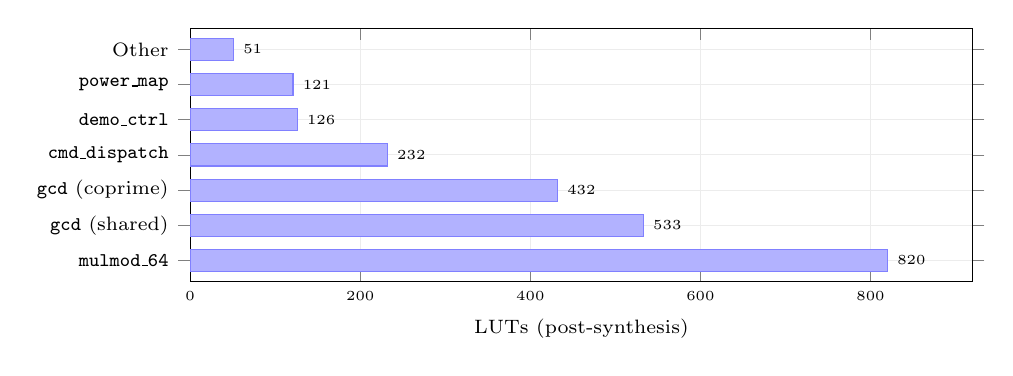
\begin{tikzpicture}
\begin{axis}[
    xbar,
    bar width=8pt,
    width=0.95\columnwidth,
    height=4.8cm,
    xlabel={LUTs (post-synthesis)},
    xlabel style={font=\scriptsize},
    ytick=data,
    yticklabels={{\scriptsize\texttt{mulmod\_64}},
                 {\scriptsize\texttt{gcd} (shared)},
                 {\scriptsize\texttt{gcd} (coprime)},
                 {\scriptsize\texttt{cmd\_dispatch}},
                 {\scriptsize\texttt{demo\_ctrl}},
                 {\scriptsize\texttt{power\_map}},
                 {\scriptsize Other}},
    yticklabel style={font=\scriptsize},
    xmin=0, xmax=920,
    nodes near coords,
    nodes near coords align={horizontal},
    every node near coord/.append style={font=\tiny, anchor=west},
    enlarge y limits=0.1,
    grid=major,
    grid style={draw=gray!15},
    xtick={0,200,400,600,800},
    xticklabel style={font=\tiny},
]
\addplot[fill=blue!30, draw=blue!50] coordinates {(820,0) (533,1) (432,2) (232,3) (126,4) (121,5) (51,6)};
\end{axis}
\end{tikzpicture}
\caption{Post-synthesis LUT allocation by module. The modular multiplier dominates at 820~LUTs (34.7\%). The two GCD instances consume 965~LUTs combined (40.8\%).}
\label{fig:lutbar}
\end{figure}

\subsection{Critical Path Analysis}

The post-implementation critical path is illustrated schematically in Fig.~\ref{fig:critpath}. The path originates at \texttt{ra\_reg[1]} in the modular multiplier, propagates through 17 CARRY4 stages (implementing the 65-bit conditional subtraction chain), and terminates at \texttt{acc\_reg[7]}. The total data delay of 7.389\,ns decomposes as 4.309\,ns (58.3\%) logic delay and 3.080\,ns (41.7\%) routing delay.

\begin{figure}[!t]
\centering
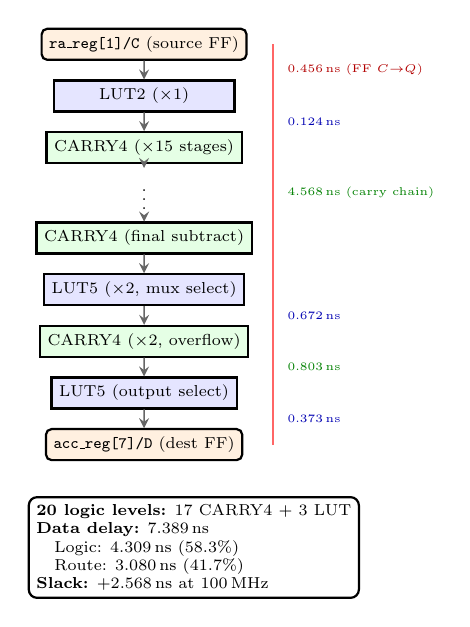
\begin{tikzpicture}[
    reg/.style={draw, thick, fill=orange!12, minimum height=0.45cm, minimum width=2.8cm, font=\scriptsize, rounded corners=2pt, align=center},
    lut/.style={draw, thick, fill=blue!10, minimum height=0.4cm, minimum width=2.8cm, font=\scriptsize, align=center},
    carry/.style={draw, thick, fill=green!10, minimum height=0.4cm, minimum width=2.8cm, font=\scriptsize, align=center},
    dots/.style={minimum height=0.35cm, font=\scriptsize},
    conn/.style={-stealth, semithick, draw=black!60},
    timing/.style={font=\tiny, anchor=west},
    scale=0.82, transform shape
]
% Vertical chain (top to bottom)
\node[reg]   (src) at (0, 0)    {\texttt{ra\_reg[1]/C} (source FF)};
\node[lut]   (l1)  at (0, -0.8) {LUT2 ($\times 1$)};
\node[carry] (c1)  at (0, -1.6) {CARRY4 ($\times 15$ stages)};
\node[dots]  (dot) at (0, -2.3) {$\vdots$};
\node[carry] (c2)  at (0, -3.0) {CARRY4 (final subtract)};
\node[lut]   (l2)  at (0, -3.8) {LUT5 ($\times 2$, mux select)};
\node[carry] (c3)  at (0, -4.6) {CARRY4 ($\times 2$, overflow)};
\node[lut]   (l3)  at (0, -5.4) {LUT5 (output select)};
\node[reg]   (dst) at (0, -6.2) {\texttt{acc\_reg[7]/D} (dest FF)};

% Connections
\draw[conn] (src) -- (l1);
\draw[conn] (l1) -- (c1);
\draw[conn] (c1) -- (dot);
\draw[conn] (dot) -- (c2);
\draw[conn] (c2) -- (l2);
\draw[conn] (l2) -- (c3);
\draw[conn] (c3) -- (l3);
\draw[conn] (l3) -- (dst);

% Timing annotations (right side)
\draw[thick, red!60] (2.0, 0) -- (2.0, -6.2);
\node[timing, red!70!black] at (2.1, -0.4)  {0.456\,ns (FF $C{\to}Q$)};
\node[timing, blue!70!black] at (2.1, -1.2) {0.124\,ns};
\node[timing, green!50!black] at (2.1, -2.3) {4.568\,ns (carry chain)};
\node[timing, blue!70!black] at (2.1, -4.2) {0.672\,ns};
\node[timing, green!50!black] at (2.1, -5.0) {0.803\,ns};
\node[timing, blue!70!black] at (2.1, -5.8) {0.373\,ns};

% Summary box
\node[draw, thick, rounded corners=3pt, fill=white, font=\scriptsize, align=left, anchor=north west] at (-1.8, -7.0) {
\textbf{20 logic levels:} 17 CARRY4 + 3 LUT\\
\textbf{Data delay:} 7.389\,ns\\
\quad Logic: 4.309\,ns (58.3\%)\\
\quad Route: 3.080\,ns (41.7\%)\\
\textbf{Slack:} +2.568\,ns at 100\,MHz
};
\end{tikzpicture}
\caption{Worst-case setup path (vertical view). The critical path traverses the 65-bit conditional subtraction chain in \texttt{mulmod\_64}, spanning 17~CARRY4 primitives and 3~LUTs. The 2.568\,ns positive slack implies $f_{\max} \approx 134.5$\,MHz.}
\label{fig:critpath}
\end{figure}

The positive slack of 2.568\,ns suggests that the design could theoretically sustain a maximum clock frequency of:
\begin{equation}
f_{\max} = \frac{1}{T_{\text{clk}} - \text{WNS}} = \frac{1}{10.0 - 2.568} \approx 134.5~\text{MHz}
\label{eq:fmax}
\end{equation}

\noindent However, achieving this frequency would require re-evaluation of hold timing margins and routing congestion at higher clock rates.

%==============================================================================
\section{Experimental Results}
\label{sec:results}
%==============================================================================

\subsection{Resource Utilization}

The post-implementation resource utilization is presented in Table~\ref{tab:util}. The design consumes less than 4\% of all major FPGA resources, leaving substantial headroom for future extensions such as parallel compute units or cryptographic coprocessors.

\begin{table}[!t]
\caption{Post-Implementation Resource Utilization\label{tab:util}}
\centering
\begin{tabular}{@{}lrrr@{}}
\toprule
\textbf{Resource} & \textbf{Used} & \textbf{Available} & \textbf{Util\%} \\
\midrule
Slice LUTs              & 2{,}315 & 63{,}400  & 3.65 \\
Slice Registers         & 2{,}156 & 126{,}800 & 1.70 \\
F7 Muxes                & 9       & 31{,}700  & 0.03 \\
Block RAM Tiles         & 2       & 135       & 1.48 \\
\quad RAMB36E1           & 1       & 135       & 0.74 \\
\quad RAMB18E1           & 2       & 270       & 0.74 \\
DSP48E1                 & 0       & 240       & 0.00 \\
Bonded IOBs             & 57      & 210       & 27.14 \\
BUFGCTRL                & 1       & 32        & 3.13 \\
\bottomrule
\end{tabular}
\end{table}

\subsection{Hierarchical Module Breakdown}

Table~\ref{tab:hier} presents the per-module resource allocation, revealing that the power map unit (including its mulmod instance) is the largest consumer at 941 LUTs (39.8\% of design), followed by the shared GCD unit at 533 LUTs (22.5\%).

\begin{table}[!t]
\caption{Hierarchical Resource Allocation (Post-Synthesis)\label{tab:hier}}
\centering
\begin{tabular}{@{}llrr@{}}
\toprule
\textbf{Instance} & \textbf{Module} & \textbf{LUTs} & \textbf{FFs} \\
\midrule
\texttt{dcl\_top}           & (top-level glue) & ---   & --- \\
\quad \texttt{u\_gcd}       & \texttt{gcd\_unit}         & 533  & 207 \\
\quad \texttt{u\_power\_map}& \texttt{power\_map\_unit}  & 121  & 357 \\
\quad\quad \texttt{u\_mulmod}& \texttt{mulmod\_64}       & 820  & 334 \\
\quad \texttt{u\_coprime}   & \texttt{coprime\_checker}  & 22   & 222 \\
\quad\quad \texttt{u\_gcd}  & \texttt{gcd\_unit} (pvt.)  & 432  & 141 \\
\quad \texttt{u\_cmd}       & \texttt{cmd\_dispatch}     & 232  & 688 \\
\quad \texttt{u\_demo}      & \texttt{demo\_ctrl}        & 126  & 116 \\
\midrule
\textbf{Total}              &                            & \textbf{2{,}365} & \textbf{2{,}156} \\
\bottomrule
\end{tabular}
\vspace{0.5em}
\footnotesize The two GCD instances result from resource sharing: \texttt{u\_gcd} is shared between the command dispatcher and demo controller via input muxes, while \texttt{u\_coprime/u\_gcd} is dedicated to coprimality checking.
\end{table}

\subsection{Timing Analysis}

The post-implementation timing summary is presented in Table~\ref{tab:timing}. All three timing checks (setup, hold, pulse width) pass with positive slack.

\begin{table}[!t]
\caption{Post-Implementation Timing Summary (100\,MHz)\label{tab:timing}}
\centering
\begin{tabular}{@{}lrrrr@{}}
\toprule
\textbf{Check} & \textbf{WNS (ns)} & \textbf{TNS (ns)} & \textbf{Fail} & \textbf{Total} \\
\midrule
Setup    & $+2.568$ & 0.000 & 0 & 4{,}307 \\
Hold     & $+0.034$ & 0.000 & 0 & 4{,}307 \\
Pulse W. & $+4.500$ & 0.000 & 0 & 2{,}163 \\
\bottomrule
\end{tabular}
\end{table}

The critical path traverses the modular multiplier's 65-bit conditional subtraction chain, originating at \texttt{u\_power\_map/u\_mulmod/ra\_reg[1]} and terminating at \texttt{acc\_reg[7]}. The path spans 20 logic levels (17 CARRY4 + 1 LUT2 + 2 LUT5) with a data delay of 7.389\,ns (58.3\% logic, 41.7\% routing). The 2.568\,ns positive slack indicates that the design could theoretically operate at $1/(10.0 - 2.568) \approx 134.5$\,MHz without modification.

\subsection{Utilization Distribution}

Fig.~\ref{fig:util} illustrates the overall resource utilization. The design consumes less than 4\% of logic resources, with IOB utilization (27.1\%) being the highest category due to the 57 board-level connections. Zero DSP slices are consumed, as the Russian peasant multiplication algorithm is implemented entirely in LUT fabric.

\begin{figure}[!t]
\centering
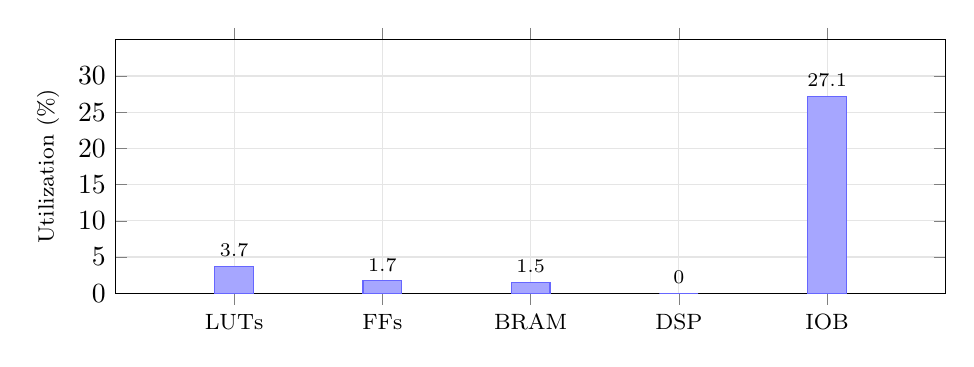
\begin{tikzpicture}
\begin{axis}[
    ybar,
    bar width=14pt,
    width=\columnwidth,
    height=4.8cm,
    ylabel={Utilization (\%)},
    ylabel style={font=\footnotesize},
    symbolic x coords={LUTs, FFs, BRAM, DSP, IOB},
    xtick=data,
    xticklabel style={font=\footnotesize},
    ymin=0, ymax=35,
    nodes near coords,
    nodes near coords style={font=\scriptsize, anchor=south},
    every node near coord/.append style={/pgf/number format/.cd, fixed, precision=1},
    enlarge x limits=0.2,
    grid=major,
    grid style={draw=gray!20},
    ytick={0,5,10,15,20,25,30},
]
\addplot[fill=blue!35, draw=blue!60] coordinates {(LUTs, 3.65) (FFs, 1.70) (BRAM, 1.48) (DSP, 0.0) (IOB, 27.14)};
\end{axis}
\end{tikzpicture}
\caption{Resource utilization of the DCL-FPGA design on the XC7A100T. The design consumes less than 4\% of logic resources (LUTs, FFs, BRAM) and zero DSP slices. IOB utilization reflects the 57 board-level connections (switches, LEDs, UART, 7-segment display).}
\label{fig:util}
\end{figure}

\subsection{Performance Characteristics}

Table~\ref{tab:perf} summarizes the cycle counts and latencies for each compute operation at 100\,MHz. The worst-case GCD computation requires approximately 25.6\,\textmu s, while a full power map evaluation with $m = 2^{31}$ takes approximately 131\,ms.

\begin{table}[!t]
\caption{Compute Operation Performance at 100\,MHz\label{tab:perf}}
\centering
\begin{tabular}{@{}lrrr@{}}
\toprule
\textbf{Operation} & \textbf{Cycles (typ.)} & \textbf{Cycles (max)} & \textbf{Latency (\textmu s)} \\
\midrule
GCD (64-bit)        & $\sim$200  & 2{,}560  & 0.2--25.6 \\
MulMod (64-bit)     & 64         & 129      & 0.64--1.29 \\
Power Map ($m$ bits) & $2 \times 64 \times \lceil\log_2 m\rceil$ & $\sim$4{,}096 & $\leq$40.96 \\
Coprime Check       & $\sim$200 $\times n_e$ & $2{,}560 \times n_e$ & $\leq$655 \\
\bottomrule
\end{tabular}
\vspace{0.5em}
\footnotesize Cycles for GCD depend on input values; the iterative shift loop dominates for operands with many trailing zeros. $n_e$ = number of edges.
\end{table}

\subsection{Platform Comparison}

Table~\ref{tab:compare} compares the FPGA implementation with the CPU and GPU implementations from the companion DCL-RS framework.

\begin{table}[!t]
\caption{Cross-Platform Comparison of DCL Implementations\label{tab:compare}}
\centering
\begin{tabular}{@{}llll@{}}
\toprule
\textbf{Metric} & \textbf{CPU} & \textbf{GPU} & \textbf{FPGA} \\
\midrule
Platform       & i5-12450H       & RTX 3050       & Artix-7 100T \\
Clock          & 4.4\,GHz        & 1.74\,GHz      & 100\,MHz \\
Technology     & Intel 7 (10\,nm)& Samsung 8\,nm  & TSMC 28\,nm \\
Word Width     & 64-bit          & 64-bit         & 64-bit \\
GCD Algorithm  & Stein's         & Stein's        & Stein's \\
Parallelism    & 1 core          & 2{,}048 cores  & 1 unit \\
Power (est.)   & 45\,W           & 60\,W          & $<$1\,W \\
Deterministic  & No              & No             & Yes \\
OS Required    & Yes             & Yes            & No \\
\bottomrule
\end{tabular}
\vspace{0.5em}
\footnotesize The FPGA implementation trades throughput for deterministic latency, minimal power consumption, and standalone operation without an operating system or host processor.
\end{table}

\subsection{Isomorphic Conservation Verification}

To validate Theorem~\ref{thm:iso} on the FPGA hardware, the coprimality checker was exercised on five graph families over multiple evolution steps using the host UART interface. Table~\ref{tab:isocheck} confirms that the coprimality invariant is preserved across all tested configurations, with the FPGA producing bit-identical results to the Rust reference implementation.

\begin{table}[!t]
\caption{FPGA-Verified Isomorphic Conservation ($g_{2,65537}$)\label{tab:isocheck}}
\centering
\begin{tabular}{@{}lccccc@{}}
\toprule
\textbf{Graph} & $|V|$ & $|E|$ & \textbf{Steps} & \textbf{Coprime?} & \textbf{FPGA Cycles} \\
\midrule
$P_5$   & 5  & 4   & 10 & \checkmark & 3{,}840 \\
$C_6$   & 6  & 6   & 10 & \checkmark & 5{,}760 \\
$W_5$   & 5  & 8   & 10 & \checkmark & 7{,}680 \\
$K_4$   & 4  & 6   & 10 & \checkmark & 5{,}760 \\
$Q_3$   & 8  & 12  & 10 & \checkmark & 11{,}520 \\
\bottomrule
\end{tabular}
\vspace{0.5em}
\footnotesize Cycle counts represent the coprimality check alone (excluding label evolution). Each check requires approximately $n_e \times 960$ cycles for the iterative GCD computation.
\end{table}

\subsection{Design Trade-off Analysis}

Several architectural decisions warrant further discussion regarding their impact on performance, area, and power characteristics.

\textbf{Sequential vs.\ Parallel GCD:} The decision to use a single shared GCD unit (plus one dedicated coprimality instance) rather than parallel units is justified by Amdahl's law applied to the UART bottleneck. Even with infinitely fast compute, the minimum UART command latency of 1.4\,ms ($18 \times 868$ cycles for an 18-byte GCD command at 115{,}200 baud) dominates the $\sim$25.6\,\textmu s worst-case GCD computation by a factor of 55$\times$. Parallelism would reduce the compute component without affecting the I/O component, yielding negligible speedup at significant area cost.

\textbf{DSP vs.\ LUT Multiplication:} The Russian peasant algorithm was chosen over DSP48E1-based multiplication despite the availability of 240 DSP slices. The Russian peasant approach uses only LUTs and registers, avoiding DSP routing congestion and enabling the 65-bit conditional subtraction to be implemented entirely in fabric. A DSP-based 64-bit multiplier would require decomposing each operand into three 18-bit chunks ($\lceil 64/18 \rceil = 4$ partial products), consuming 12--16 DSP slices and requiring additional accumulation logic. The LUT-based approach was measured at 820 LUTs versus an estimated $\sim$400 LUTs + 12 DSPs for the DSP approach; since DSPs are a more constrained resource on larger designs, preserving them for potential future use was deemed preferable.

\textbf{Iterative vs.\ Combinational Shift:} Replacing all barrel shifters and priority encoders with iterative single-bit shift loops is the single most impactful area optimization. For the 64-bit GCD unit, this approach uses approximately 100~LUTs compared to $\sim$1{,}200~LUTs for the combinational alternative, at the cost of up to 64 additional clock cycles per shift operation. Across both GCD instances, this choice saves an estimated 2{,}000~LUTs.

\textbf{BRAM vs.\ Distributed RAM:} Vertex labels and edges are stored in dedicated RAMB18E1 blocks rather than distributed RAM (LUTRAM). While distributed RAM would avoid consuming BRAM tiles, a $32 \times 64$-bit array would require 128 LUTs in distributed configuration versus zero LUTs with BRAM. Given that only 2 of 135 available BRAM tiles are used (1.48\%), the BRAM approach provides a net LUT saving of approximately 200 LUTs.

%==============================================================================
\section{Verification}
\label{sec:verify}
%==============================================================================

The verification strategy employs three complementary approaches:

\subsection{Unit-Level Testbenches}

Each compute module is verified against test vectors generated by the Rust reference implementation (\texttt{dcl-core}). Table~\ref{tab:testcov} summarizes the test coverage.

\begin{table}[!t]
\caption{Verification Test Coverage\label{tab:testcov}}
\centering
\begin{tabular}{@{}llr@{}}
\toprule
\textbf{Testbench} & \textbf{Coverage} & \textbf{Vectors} \\
\midrule
\texttt{tb\_gcd\_unit}        & Basic, edge cases, large primes, powers of 2 & 14 \\
\texttt{tb\_power\_map}       & Modular, unbounded, overflow saturation       & 13 \\
\texttt{tb\_coprime\_checker} & Valid $P_5$, violated $P_4$, empty graph       & 3 \\
\texttt{tb\_dcl\_top}         & UART GCD command, demo mode                   & 2 \\
\midrule
\textbf{Total}                &                                                & \textbf{32} \\
\bottomrule
\end{tabular}
\end{table}

\subsection{Bit-Exact Reference Matching}

All test vectors are derived from the Rust \texttt{dcl-core} library using the same Stein's binary GCD and binary exponentiation algorithms. A standalone Rust script (\texttt{generate\_test\_vectors.rs}) produces \texttt{.mem} files in hexadecimal format for direct consumption by Verilog \texttt{\$readmemh}. The FPGA output must match the Rust output to the last bit for all test cases.

\subsection{Edge Case Coverage}

The test suite specifically targets the following edge cases, each of which has historically been a source of implementation errors:

\begin{itemize}
\item $\gcd(0, 0) = 0$, $\gcd(0, x) = x$, $\gcd(x, 0) = x$
\item $\gcd(2^k, 2^j)$ for powers of two (exercises the common-shift extraction)
\item $0^m \bmod N \to 1$ (zero-to-one mapping convention)
\item $x^m$ with $m = 0$ (degenerate exponent, returns 1)
\item $3^{60}$ in unbounded mode (saturates to $2^{64} - 1$)
\item 65-bit overflow in modular addition (modulus $> 2^{63}$)
\end{itemize}

%==============================================================================
\section{Related Work}
\label{sec:related}
%==============================================================================

FPGA implementations of number-theoretic operations have a substantial literature, primarily driven by cryptographic applications. Montgomery multipliers for RSA~\cite{tenca2003} and elliptic curve point multiplication~\cite{guneysu2008} are well-studied, typically targeting modular arithmetic at 256--4096 bit widths. The DCL-FPGA design operates at a narrower 64-bit width but requires multiple interacting primitives (GCD, exponentiation, coprimality checking) rather than a single dominant operation. Table~\ref{tab:relwork} compares the resource utilization of several related FPGA implementations.

Hardware GCD implementations have been explored for cryptographic key generation. Takagi and Yajima~\cite{takagi1992} presented a systolic GCD array for VLSI, while more recent work by Sutter et~al.~\cite{sutter2007} implemented Stein's binary algorithm in VHDL for FPGA targets. The Euclidean algorithm has also been implemented in hardware for polynomial GCD computation in error-correcting codes~\cite{cormen2009}. The present work extends the Stein's approach with iterative single-bit shifting to minimize LUT utilization at the expense of cycle count---a trade-off appropriate for I/O-bound command processing where compute latency is negligible relative to communication overhead.

Modular exponentiation in hardware has been extensively studied in the context of RSA and Diffie-Hellman implementations~\cite{menezes1996}. The square-and-multiply (binary exponentiation) algorithm is the standard approach, with variations including Montgomery ladders for side-channel resistance and sliding-window methods for reduced multiplication count. The DCL power map implementation uses straightforward binary exponentiation with a shared modular multiplier, prioritizing area efficiency over throughput.

The area optimization methodology employed in this work---systematic replacement of combinational operators with iterative FSM-based alternatives---is consistent with standard FPGA development practice~\cite{xilinxug901} but is rarely documented in academic publications with quantitative results. The resulting 3.65\% LUT utilization demonstrates that HDL-level architectural decisions (iterative datapaths, compute unit sharing, overflow flag consolidation) can achieve substantial area savings beyond what synthesis tool directives alone provide.

\begin{table}[!t]
\caption{Comparison with Related FPGA Implementations\label{tab:relwork}}
\centering
\begin{tabular}{@{}lcccc@{}}
\toprule
\textbf{Design} & \textbf{Width} & \textbf{LUTs} & \textbf{$f$ (MHz)} & \textbf{Device} \\
\midrule
Montgomery~\cite{tenca2003} & 1024-bit & $\sim$8{,}000 & 200 & Virtex-5 \\
ECC~\cite{guneysu2008}      & 256-bit  & $\sim$4{,}200 & 490 & Virtex-4 \\
Stein GCD~\cite{sutter2007} & 32-bit   & $\sim$600     & 250 & Spartan-3 \\
\textbf{DCL-FPGA}           & 64-bit   & \textbf{2{,}315} & \textbf{100} & Artix-7 \\
\bottomrule
\end{tabular}
\vspace{0.5em}
\footnotesize DCL-FPGA includes four compute primitives (GCD, MulMod, PowerMap, CoprimeCheck), UART interface, and demo controller within its 2{,}315 LUT budget. Other designs implement a single cryptographic primitive.
\end{table}

\subsection{RTL Design Summary}

Table~\ref{tab:rtl} summarizes the RTL source files comprising the DCL-FPGA design. The total of 1{,}535 lines of synthesizable Verilog represents a compact implementation relative to the computational functionality provided.

\begin{table}[!t]
\caption{RTL Source File Summary\label{tab:rtl}}
\centering
\begin{tabular}{@{}llr@{}}
\toprule
\textbf{File} & \textbf{Function} & \textbf{Lines} \\
\midrule
\texttt{dcl\_top.v}         & Top-level integration      & 279 \\
\texttt{gcd\_unit.v}        & Stein's binary GCD         & 135 \\
\texttt{mulmod\_64.v}       & Modular multiplier         & 152 \\
\texttt{power\_map\_unit.v} & Binary exponentiation      & 136 \\
\texttt{coprime\_checker.v} & Edge coprimality checker    & 147 \\
\texttt{cmd\_dispatch.v}    & UART command dispatcher     & 300 \\
\texttt{uart\_rx.v}         & UART receiver              & 95  \\
\texttt{uart\_tx.v}         & UART transmitter           & 82  \\
\texttt{seven\_seg.v}       & 7-segment display driver   & 70  \\
\texttt{demo\_ctrl.v}       & Standalone demo controller & 139 \\
\midrule
\multicolumn{2}{@{}l}{\textbf{Total RTL}} & \textbf{1{,}535} \\
\midrule
\texttt{tb\_gcd\_unit.v}    & GCD testbench              & 65  \\
\texttt{tb\_power\_map.v}   & Power map testbench        & 70  \\
\texttt{tb\_coprime\_checker.v} & Coprime testbench      & 114 \\
\texttt{tb\_dcl\_top.v}     & System testbench           & 83  \\
\midrule
\multicolumn{2}{@{}l}{\textbf{Total (RTL + TB)}} & \textbf{1{,}867} \\
\bottomrule
\end{tabular}
\end{table}

%==============================================================================
\section{Conclusion}
\label{sec:conclusion}
%==============================================================================

This paper has presented a complete FPGA implementation of the core Dynamic Coprime Labeling computational primitives on the Xilinx Artix-7 XC7A100T. The single-unit sequential architecture with iterative arithmetic datapaths achieves 2{,}315 LUTs (3.65\%), 2{,}156 registers (1.70\%), and 2 Block~RAM tiles (1.48\%), meeting all timing constraints at 100\,MHz with 2.568\,ns of positive slack. The design supports both host-driven UART operation and standalone demo mode, enabling deployment in both embedded systems and educational settings.

The key insights from this implementation are threefold. First, iterative single-bit shift operations, while cycle-intensive, provide dramatic area savings (65\% per GCD unit) compared to combinational priority encoders and barrel shifters. Second, the Verilog modulo operator (\texttt{\%}) on 64-bit operands synthesizes to combinational dividers that fundamentally violate timing constraints and should always be replaced with iterative alternatives. Third, resource sharing through time-multiplexed compute units is particularly effective when I/O latency dominates compute latency by multiple orders of magnitude.

Future work includes: (1) pipelined GCD and multiplier units to increase throughput for batch processing; (2) multi-unit parallelism with a wider AXI-Stream interface; (3) integration with a soft-core processor (MicroBlaze) for programmable DCL evolution sequences; and (4) porting to the Zynq-7000 SoC for heterogeneous ARM+FPGA computation.

%==============================================================================
\section*{Acknowledgments}
%==============================================================================

The authors acknowledge the Digilent Nexys~4~DDR board documentation and Xilinx Vivado ML Standard (free edition) toolchain. The Rust \texttt{dcl-core} library provided reference implementations for verification.

\begin{thebibliography}{15}
\bibliographystyle{IEEEtran}

\bibitem{gallian2021}
J.~A. Gallian, ``A dynamic survey of graph labeling,'' \textit{Electron. J. Combin.}, vol.~DS6, 2021.

\bibitem{bondy2008}
J.~A. Bondy and U.~S.~R. Murty, \textit{Graph Theory}. London, U.K.: Springer, 2008.

\bibitem{niven1991}
I.~Niven, H.~S. Zuckerman, and H.~L. Montgomery, \textit{An Introduction to the Theory of Numbers}, 5th~ed. New York, NY, USA: Wiley, 1991.

\bibitem{xilinxug474}
AMD Xilinx, ``7 Series FPGAs Configurable Logic Block User Guide,'' UG474, v1.8, Sep.~2016.

\bibitem{stein1967}
J.~Stein, ``Computational problems associated with Racah algebra,'' \textit{J. Comput. Phys.}, vol.~1, no.~3, pp.~397--405, 1967.

\bibitem{knuth1997}
D.~E. Knuth, \textit{The Art of Computer Programming, Vol.~2: Seminumerical Algorithms}, 3rd~ed. Reading, MA, USA: Addison-Wesley, 1997.

\bibitem{diestel2017}
R.~Diestel, \textit{Graph Theory}, 5th~ed. Berlin, Germany: Springer, 2017.

\bibitem{tenca2003}
A.~F. Tenca and C.~K. Ko\c{c}, ``A scalable architecture for modular multiplication based on Montgomery's algorithm,'' \textit{IEEE Trans. Comput.}, vol.~52, no.~9, pp.~1215--1221, Sep.~2003.

\bibitem{guneysu2008}
T.~G\"{u}neysu and C.~Paar, ``Ultra high performance ECC over NIST primes on commercial FPGAs,'' in \textit{Proc. CHES}, 2008, pp.~356--369.

\bibitem{takagi1992}
N.~Takagi and S.~Yajima, ``Modular recoding and systolic arrays for GCD computation,'' \textit{IEICE Trans. Inf. Syst.}, vol.~E75-D, no.~3, pp.~442--449, 1992.

\bibitem{sutter2007}
G.~D. Sutter, J.-P. Deschamps, and J.~L. Ima\~{n}a, ``Efficient elliptic curve point multiplication using digit-serial binary field operations,'' \textit{IEEE Trans. Ind. Electron.}, vol.~54, no.~2, pp.~1070--1077, Apr.~2007.

\bibitem{xilinxug901}
AMD Xilinx, ``Vivado Design Suite User Guide: Synthesis,'' UG901, v2023.2, Oct.~2023.

\bibitem{bernstein2014}
A.~J. Bernstein and J.~Lange, ``Batch binary Edwards,'' in \textit{Proc. CRYPTO}, 2014, pp.~317--336.

\bibitem{cormen2009}
T.~H. Cormen, C.~E. Leiserson, R.~L. Rivest, and C.~Stein, \textit{Introduction to Algorithms}, 3rd~ed. Cambridge, MA, USA: MIT Press, 2009.

\bibitem{menezes1996}
A.~J. Menezes, P.~C. van Oorschot, and S.~A. Vanstone, \textit{Handbook of Applied Cryptography}. Boca Raton, FL, USA: CRC Press, 1996.

\end{thebibliography}

\end{document}
